\chapter{Introduction}

Most of Internet traffic is content, and most of Internet connected hosts are mobile. A key example of the content-dominated nature of Internet is that online video accounts for nearly 70\% of traffic today and is expected to grow to nearly 80\% by 2018 \cite{cisco-videogrowth}. The evidence of a highly mobile Internet is that 5B mobile devices connect to the Intenet today and thet generate more traffic than wired devices \cite{cisco-vni}.

%It is estimated that a vast majority of network traffic on the Internet is content, with videos alone expected to account for 80\% of all traffic by 2018 . By 2020, the number of Internet connected mobile end hosts is expected to grow to nearly 10 billion and the total traffic originated by mobiles is poised to approach that by wired devices .

A content-dominated, highly mobile Internet needs several forms of infrastructure support. It needs network switches and links with sufficient capacity to carry traffic to end users. It needs servers to sustain and accelerate delivery of content. It also needs an infrastructure to help establish and maintain connections in the presence of high network moblity or changing of addresses. The focus of this thesis is to design \emph{services} that manage the resources on such infrastructures towards achieving the desired goals.

%the design of services that manage the infrastructure resources achieve the desired goals.
%This thesis focuses on the design of services that manage the infrastructure resources achieve the desired goals.

%The focus of this thesis is the design of these infrastructure 

%In the presence of frequent network mobility or changing addresses, infrastructure support becomes necessary for . This thesis focuses on the design of services that manage the infrastructure resources achieve the desired goals.

\section{Infrastructure characteristics}
%	Characteristics of infrastructure}

Our service designs are strongly influenced by the following characteristics of the infrastructures supporting a content-dominated, highly mobile Internet.

\textbf{Cost-intensive} There is a substantial captial and operational cost in running a large-scale infrastructure \cite{greenberg2008cost}, and which causes a sigificant reduction in the profit margins of the infrastructure owner. A prominent example of low-profit infrastructures are Internet service provider networks \cite{isp-low-profit}. Cost reduction while meeting performance and other constraints is a central design problem that we address in this thesis. 

\textbf{Geo-distributed:} These infrastructures are often highly geo-distribtued, e.g., a large internet service provider (ISP) or a content delivery network (CDN) has Points-of-Presence (POP) at hundreds of locations \cite{dilley2002globally}. Thus, it is necessary that services be designed to leverage geo-distributed deployments for reducing user-perceived latencies.

\textbf{Locality-exhibiting workload:} Real-worlds workloads served by these infrastructures tend to exhibit significant geographic and temporal locality \cite{NCDN, youtubeUGC, vodP2Pbenefit, cellularvideotraffic}. Exploiting locality of demand to reduce infrastructure cost as well as user-perceived latencies is a key focus in our service designs.

\section{Degrees of freedom in infrastructure service design} 

Due to their geo-distributed deployment, these infrastructure services commonly make three sets of decisions: \emph{content placement}, \emph{request redirection}, and \emph{network routing}. As each of these decisions can be made relatively independently of others, we call them ``degrees of freedom'' available to a service.

\begin{itemize}
	\item
	\textbf{Content placement} selects the locations at which a content is placed. Its objective  is to balance resource cost of keeping multiple content replicas with the benefits of improved availability and reduced user-perceived latency.
	\item
	\textbf{Request redirection} selects a location to send a request to, with a preference for selecting a location that is nearby and has sufficient resources to serve the request.
	\item
	\textbf{Network routing} (or \textbf{traffic engineering}) selects the physical paths between nodes in the network based on topoology and traffic demand patterns. A key goal is to avoid congestion hotspots in the network.
\end{itemize}


\section{Thesis statement}

\emph{Content placement is a more powerful factor that request redirection and network routing in determining the cost, performance and energy-related metrics for infrastructures supporting a content-dominated, highly mobile Internet.}

\section{Why placement is more powerful than redirection, routing}

Geo-distribtued infrastructure and workload locality makes content placement a powerful degree of freedom. Workload locality implies that a content is typically popular in only a few regions at any given time, and as a result only a few replicas of a content are sufficient to reduce user-perceived latency for most users. Further, the geo-distribued infrastructure enables these few replicas to be placed close to regions of demand, thereby achieving a good tradeoff between user-perceived latency and infrastructure cost. We illustrate with a couple of examples why placement can be a more powerful degree of freedom than redirection and routing in designing infrastructure services.


\begin{figure}
	
	\centering
	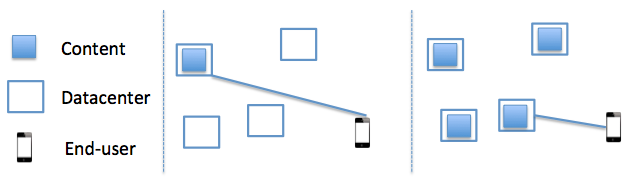
\includegraphics[scale=0.5]{fig/placement-vs-redirection.png}
	\caption{Placement vs. redirection: Content placement creates options for the redirection scheme to choose a nearby location for reducing user-perceived latencies.}	
	\label{fig:placement-redirection}
\end{figure}


\textbf{Placement vs. redirection:} Suppose a user requests a content that is placed only at a remote location as in Figure \ref{fig:placement-redirection} (left). Irrespective of the redirection scheme, a user will observe high latencies to fetch content from the remote location. Placement is more powerful that redirection becasue it can create more options for the redirection scheme, enabling it to choose a location that is nearby as shown in Figure \ref{fig:placement-redirection} (right). Thus, effective placement is a pre-requisite for a redirection scheme to provide low latencies.


%We briefly explain the \emph{traffic engineering} problem that is pertinent to our discussion of placement vs. routing. Traffic engineering computes network routing based on inputs of are the network topology, link capacities, and a \emph{traffic matrix}. A traffic engineering scheme computes routing to satisfy traffic demands while optimizing a cost function dependent on link utilization. For example, a common cost function is the maximum link utilization, MLU \cite{rexford}. 


\textbf{Placement vs. routing:} Content placement is more powerful than routing because it can change the \emph{traffic matrix} for which the routing is to be computed. A traffic matrix is a 2-dimensional matrix representing the demand in the network. The $i,j$-th entry in this matrix is the traffic from node $i$ to node $j$ in the network topology \cite{fortz2000internet}.  Let us take an example traffic matrix for which routing is to be computed (Figure \ref{fig:placement-routing}). Content placement can turn any traffic matrix into a null matrix (one whose all entries are zero) provided all content that a node in a network needs is placed at the same node. Such a placement obviates the need to send traffic to any other node, and therefore makes routing a trivial problem. While this is an extreme example, and one may not have sufficient resources to place content at all locations in the network, this example demonstrates that the ability to change the traffic matrix makes content placement more powerful than routing.

\begin{figure}
	\centering
	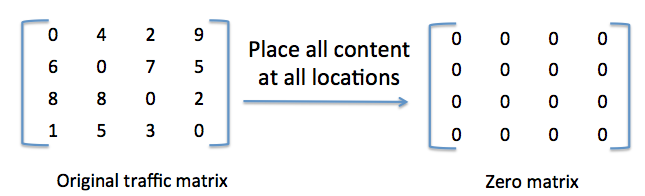
\includegraphics[scale=0.4]{fig/placement-vs-routing.png}
	\caption{Placement vs. routing: content placement is more powerful than routing since it can change the  traffic matrix itself.}
	\label{fig:placement-routing}
\end{figure}


\section{Research overview}

We consider three types of infrastructures in this thesis.

\begin{description}
	\item[Internet service provider (ISP):] ISPs perform traffic engineering to achieve several objectives such as cost and congestion reduction, fault tolerance etc. As explained in Section \ref{sec:intro-te}, our work designs and evaluates traffic engineering in content-dominated ISP networks while accounting for its interaction with placement and redirection schemes. 
	\item[Global name service (GNS):] GNS can enable establishing and maintaining connections between mobile entities on the Internet. As explained in Section \ref{sec:intro-gns}, our name service design, Auspice, meets the challenge posed by high mobility, which is to return up to date addresses for billions of mobile names with frequently changing network address.
	\item[Content datacenter (CDC):] Content datacenters are used to store and serve content to end users. As explained in Section \ref{sec:intro-cdc}, our work quantifies the tradeoff between user-perceived performance and energy savings achieved via a coordinated consolidation of servers and switches, and presents the design and implementation of a system to leverage this tradeoff.
\end{description}

\subsection{Traffic engineering in content-dominated networks}
\label{sec:intro-te}
In an ISP network with content-dominated traffic, traffic engineering decisions are not isolated from content placement and request redirection. As above examples show, content placement and request redirection determine the traffic matrix and hence influence traffic engineering. A key question therefore is how should traffic engineering be done in light of the interaction between placement, redirection and routing.

We address the above question in two scenarios. The first scenario in a more common occurence in present day Internet, in which an ISP has little control over placement and redirection. The second scenario is motivated by a recent, potentialy transformative trend: Network CDNs (NCDNs) -- CDNs deployed by ISPs on their infrastructures. Unlike traditional ISPs, NCDNs enjoy full control over placement, redirection and routing on their networks.

\subsubsection{ISP network with content location diversity}

We model a content-dominated ISP network by accounting for its content \emph{location diversity} -- the presence of content at multiple network locations, and the ability of end-users to download content from those locations. Location diversity is enabled by several types of applications and services, such as CDNs, P2P, mirrored websites. We create location diversity using a simple content placement scheme -- randomly placing content at multiple locations --, to reflect the limited control of ISPs on content placement in their networks. 

%We further assume that users can download content in parallel from all locations. 

Our work presents an experimental comparison of several classes of traffic engineering schemes using data from real ISP topologies and traffic matrices. Our key findings are as follows: (1) All traffic engineering schemes, including shortest-path routing, multiprotocol label switching routing, routing that is robust to unpredictable variations as well as optimal traffic engineering, achieve similar application performance and network capacity.   (2) Even a static shortest-path routing, or in other words a ``no'' traffic engineering  scheme is at most 30\% sub-optimal in terms of network capacity. Overall, these results suggest that even a limited placement flexibility reduces the value of sophisticated traffic enginering schemes, e.g., optimal traffic engineering, over simpler traffic engineering schemes, e.g., shortest path routing. These results are further strengthed in the case of an NCDN where the content placement flexibility is even greater.


\subsubsection{Network CDNs}

There are strong economic factors motivating ISPs to transform into NCDNs for delivering content to users on its network: %falling bandwidth prices due to competition and technology trends, 
potential sources of revenue by selling content-based services to end-users, easy availability of CDN technology in the form of licensed and managed CDNs and reduction in backbone traffic due to content caching via NCDNs \cite{telco-cdn-arguments}. These factors have motivated more than 30 ISPs to deployed NCDNs on their network.

NCDNs represent a paradigm shift in which both content delivery and traffic engineering is handled by a single entity. This change affects the metrics of interest of an NCDN as well the techniques an it can use. While a traditional ISP is concerened with traffic enginerring related objectives such as network link utilization, and a traditional CDN is concered with optimizing user-perceived performance, an NCDN is concered with both these metrics. While a traditional ISP can decide network routing and a traditional CDN can decide placement and redirection, but only an NCDN decides placement, redirection and routing. Besides using existing techniques to handle these tasks independently, an NCDN has the option of jointly optimizing these decisions as well. 

%An NCDN controls content delivery related decisions such as placement and redirection in addition to network routing. 

Our contribution is to evaluate existing schemes as well as a new joint optimization scheme for NCDNs based on real network topologies and extensive real world content access traces from Akamai CDN. The schemes we evaluate include (1) a simple caching scheme for placement and a static-shortest path routing, (2) a joint optimization based on historic demand patterns and (3) an ideal joint optimization with future knowledge of content demand. Of particular interest to NCDNs are demand-oblivious schemes such as the first scheme, as they make placement and routing decisions without measurement of content demand and simplify network management for the operators.


Our study presents two main conclusions. First, simple demand oblivious schemes perform well. Due to poor predictability of content demand and the churn in content workloads, a history-based joint optimization scheme performs much worse than the simple demand-oblivious scheme. The demand-oblivious scheme performs close to an ideal joint-optimization strategy with knowledge of future content demand, largely because the caching scheme achieves high cache hit rates from caches placed inside the network. Second, optimizing routing matters little in NCDNs: whether a static shortest-path routing or a routing optimized based on measured traffic demands is used along with a caching scheme, the network cost differs by less than 10\%.  Overall, these result show the importance of content placement over routing in NCDNs. 



\subsection{Global name service for highly mobile Internet}
\label{sec:intro-gns}


\tbd{write motivation here.The effects of Inernet's poor support for mobility are present everywhere:}

A key reason for Internet's poor support for moblity is that communication on the Internet is based on IP addresses that keep changing due to mobility. On the other hand, what remains unchanged is the name or identity of communication end-points. If we can enable communication over names, we can handle mobility. A  global name service (GNS) enable such a name-based communication by maintaining an up-to-date mapping from names to network addresses for all names. Figure \ref{fig:gns-example} illustrates the use of GNS in handling mobility. A mobile user Bob updates the GNS with its new address soon after changing its network address. Alice obtains Bob's new address from the GNS and is able to establish connection with Bob despite Bob's mobilty.

\begin{figure}
	\centering
	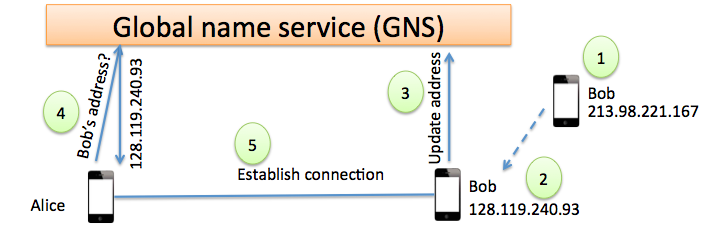
\includegraphics[scale=0.4]{fig/gns-example.png}
	\label{fig:gns-example}
	\caption{A global name service helps establish and maintain connections between mobile entities by keeping an up-to-date mapping from their names to their network addresses. \tbd{add bob's mobility to figure}}
\end{figure}

To appreciate the challenges in implementing such a GNS, we discuss the limitation of Internet's existing naming service DNS as a solution for mobility.
\begin{description}
	\item[Passive caching:] 
	DNS relies heavily on passive caching based on TTLs for reducing both system load and client-perceived latency. However, high mobility severely limits effectiveness of TTL-caching. Handling mobility requires up-to-date responses, so the load and client-perceived latency increase with the mobility rate irrespective of the TTL.
	\item[Static placement:] 
	Under high mobility, the latency to an authoritative name server determines user-perceived query latency in the common case. Today, authoritative name server locations are chosen statically irrespective of where the query demand is coming from, which could result in highly sub-optimal query latencies for users querying the name service from a location distant from the statically placed replicas. 
	\item[Hierarchical names:]
	The main proposal to enhance DNS's security, DNSSEC, is dependent on a single root of trust due to DNS's hierarchical design. A root that is tightly controlled today by ICANN and the US Department of Commerce, a state-of-affairs that is inherently anti-competitive and geo-politically problematic. \tbd{clarify more} 
\end{description}

While the first two problems are related to authoritative name servers and can be addressed within the scope of current DNS, the third issue requires a clean slate redesign of the naming system. Below, we first discuss our naming system design followed by a new authoritative name service design.



%Our work makes two main contributions towards addressing the challenges of designing a global name service for high mobility. 

\textbf{Global naming system:} We present a clean-slate naming system design that is incompatible with the existing DNS but improves upon DNS's design in two aspects. First, it supports multiple roots of trust as a part of the naming system, thereby addressing the single root of trust problem in DNS. Second, it supports name-to-address resolution for arbitrary names unlike DNS, which restricts names to be hierarchical. In doing so, our naming system gives applications the full flexibility in choosing names. 

\textbf{Auspice name resolution service:} \tbd{revise this paragraph, shorten and connect} A key component of our naming system is Auspice: a scalable geo-distributed service for mapping names to network addresses under high mobility. A key decision in Auspice's design is that of placement of name records that store the name-to-address mapping. The placement problem is challenging due to a fundamental cost-vs.-performance trade-off: placing name record at multiple locations improves latency of content accesses but increases update propagation costs of keeping consistent replicas. To address this challenge, Auspice name resolution service infers pockets of high demand for a name and uses a heuristic placement strategy that selects both the number and location of the replicas in a demand-aware manner to provide low request latency, low update cost, and high availability.  We extensively evaluate Auspice for an expected workload of a global name service and show that it significantly outperforms both commercial managed DNS services as well as DHT-based replication alternatives to DNS. Auspice is deployable in the Internet today as a scalable managed DNS provider, potentially enhacing support for mobility in the present day Internet as well.

\subsection{Energy optimization in content datacenters}
\label{sec:intro-cdc}
Energy use is a key component of operational costs of \emph{content datacenters (CDCs)}, datacenters that are used for storing and serving content to end-users. CDCs can potentially reduce their energy use via consolidation of servers and switches, but in doing so, they risk inflating end-user response times potentially leading to SLA violations. Our primary contribution is to quantify the tradeoff between energy savings via consolidation and response times in CDCs, and the design and implementation of Shrink, a system that aggressively leverages this tradeoff in order to yield significant savings in energy use in CDCs while affecting user-perceived response times in a controlled manner. To our knowledge, Shrink is the first system to consolidate servers and switches in a coordinated manner, an approach that reduces network energy use by up to 42\% compared to network-unaware server consolidation schemes. Our evaluation of Shrink using a workload from a large CDN's datacenter shows that Shrink can reduce energy use by 35\% over a scheme provisioned for the peak demand, while increasing the mean, 95th and 99th percentile response times by 8\%, 3\% and 15\% respectively.



\section{Thesis organization}

The thesis is organized intro three parts in correspondence with the three topics of our research.

Chapter \ref{ch:te-background}, Chapter \ref{ch:beyondmlu} and Chapter \ref{ch:ncdn} present our research on traffic engineering in content-dominated networks. Chapter \ref{ch:te-background} presents background on traffic engineering, content delivery and the interaction between them. Chapter \ref{ch:beyondmlu} presents a comparison of traffic engineering schemes in a network with location diversity of content. Chapter \ref{ch:ncdn} designs and evaluates traffic engineering and content delivery schemes in a Network CDN.

Chapter \ref{ch:intro-auspice} presents the design, implementation and evaluation of a global name service for a highly mobile Internet.

Chapter \ref{ch:shrink} presents the design, implementaiton and evaluation of Shrink - a system for reducing energy use of content datacenters via server consolidation.

\section{Previous publications and collaboration}

\textbf{Chapter \ref{ch:beyondmlu}} revises a previous publication: A. Sharma, A. Mishra, V. Kumar, A. Venkataramani. Beyond MLU: An Application-Centric Comparison of Traffic Engineering Schemes. \emph{Proc. IEEE INFOCOM, April 2011}. Aditya Mishra and Vikas Kumar provided invaluable support in performing experiments for this work.

\textbf{Chapter \ref{ch:ncdn}} revises a previous publication: A. Sharma, A. Venkataramani, R. Sitaraman. Distributing Content Simplifies ISP Traffic Engineering. \emph{Proc. ACM SIGMETRICS, June 2013}. Ramesh Sitaraman provided access to Akamai datasets for this work. A realistic experimental evaluation would not have been possible without these datasets.

\textbf{Chapter \ref{ch:intro-auspice}} revises a previous publication: A. Sharma, X. Tie, H. Uppal, D. Westbrook, A. Venkataramani, A. Yadav. A Global Name Service for a Highly Mobile Internetwork. \emph{Proc. ACM SIGCOMM, August 2014}. 
This work also appears in Xiaozheng Tie's thesis, which describes the same placement algorithm and a simulation-based evaluation of the algorithm. The new material in this chapter includes (1) mechanisms to provide consistency of data and (2) experiments with an implementation of the placement algorithm in an emulation testbed and a geo-distributed testbed. Both Xiaozheng Tie and Hardeep Uppal have contributed to the placement algorithm. Hardeep Uppal, David Westbrook and Arun Venkataramani have contributed in implementing the \auspice\ system.

